% !TEX root = Projektdokumentation.tex

\newglossaryentry{Usability-Test}{name={Usability-Test},description={Probanden aus der Zielgruppe der Anwendung werden Aufgaben gestellt, welche sie mit der bestehenden Anwendung lösen sollen. Dabei wird untersucht, welcher Weg zur Lösung der Aufgabe eingeschlagen wird und wo dabei Probleme auftauchen.}}

\newglossaryentry{Wireframes}{name={Wireframes},description={Die Visualisierung stellt die Seitenstruktur und Featureumsetzung sehr grob und schematisch dar. Das Wireframe wird in schwarz-weiss-grau angefertigt und gleicht dadurch einer Skizze oder Bleistiftzeichnung. Dieses Art der Visualisierung ist sehr schnell, einfach und günstig zu erstellen. Dazu genügt Papier und Bleistift oder eine entsprechende Wireframe-Software.}}

\newglossaryentry{User Interface}{name={User Interface},description={Unter einer Benutzeroberfläche oder Benutzerschnittstelle (UI) versteht man die Art und Weise, wie Befehle und Daten in den Computer eingegeben werden. Die Benutzeroberfläche ist die Schnittstelle zwischen Computer und Mensch. \cite{itWissen_benutzeroberflache}}}

\newglossaryentry{Commit}{name={Commit},description={Vorgang bei einem Versionsverwaltungssystem, um neuen oder geänderten Quellcode einzuspielen. \cite{commit}}}

\newglossaryentry{Refactoring}{name={Refactoring},description={\begin{quote}
			Mit Refactoring bezeichnet man die Überarbeitung der Struktur einer Software, ohne dass sich deren Verhalten nach außen ändert.
		\end{quote} \cite{refactoring}}}

\newglossaryentry{Add-on}{name={Add-on},description={Erweiterung eines bestehenden Systems}}

\newacronym{CN1}{CN1}{Computernetze 1}
\newacronym{UI}{UI}{User Interface}
\newacronym{CI}{CI}{Continuous Integration}


%Qualitätsmanagement: Messungen, Tests, Usability Tests, Code Review usw. (mit vollständiger Beschreibung der Anordnungen und Rahmenbedingungen)

\section{Usability}
\label{sec:usability}
Im Internet gibt es zahlreiche Online-Quizzes, auch für das schulische Umfeld. Damit Mobile Quiz häufig und gerne genutzt wird, gibt es einige Faktoren zu beachten. \cite{marketingfire.de} Dazu zählen unter anderem das Design und die Strukturierung der Seite. \\

Wie gut die bestehende Mobile Quiz - Version in diesen Bereichen abschneidet, wurde mit \gls{Usability-Test}s herausgefunden. Davon wurden zwei Durchführungen gemacht, wobei die erste zu Beginn der Arbeit dabei half, Schwierigkeiten in der Bedienung offenzulegen. Anschliessend flossen die Ergebnisse in die Aufgabenstellung mit ein. Am Ende der Arbeit fand dann die zweite Durchführung statt, um zu messen, welche Fortschritte durch die Arbeit gelungen sind.

\subsection{Methoden}
Bei den \gls{Usability-Test}s zu Beginn der Arbeit nahmen drei Studenten der \acrfull{CN1}-Vorlesung, ein Student aus der Raumplanung sowie ein Student aus dem 5. Semester Informatik teil, was der Zielgruppe von Mobile Quiz entspricht. Abgesehen vom Informatik-Student aus dem 5. Semester hatten die Teilnehmer noch wenig bis gar keine Erfahrung mit Mobile Quiz gesammelt.

Bei der Durchführung wurden die Teilnehmern in Situationen hineinversetzt, welche bei der Benutzung von Mobile Quiz oft vorkommen (siehe Usability-Test\_Aufgabenstellung auf Seite \hyperlink{page.\getpagerefnumber{pdf:UTAS1}}{\getpagerefnumber{pdf:UTAS1}}). Die Teilnehmer wurden dabei eins zu eins beobachtet und Schwierigkeiten oder Abweichungen von den Erwartungen notiert. Die Gesamtauswertung wurde anschliessend in einem separaten Dokument festgehalten (siehe Usability-Test\_Auswertung\_Durchführung1 auf Seite \hyperlink{page.\getpagerefnumber{pdf:UTAW1}}{\getpagerefnumber{pdf:UTAW1}}).

Am Ende der Arbeit wurden eine Auswahl der gleichen Tests nochmals durchgeführt (siehe Usability-Test\_Aufgabenstellung2 auf Seite \hyperlink{page.\getpagerefnumber{pdf:UTAS2}}{\getpagerefnumber{pdf:UTAS2}}). Es nahmen dabei drei Informatikstudenten aus dem Modul \gls{CN1} teil. Aus dieser Durchführung wurden die Auswertungen ebenfalls niedergeschrieben (siehe Usability-Test\_Durchführung2 auf Seite \hyperlink{page.\getpagerefnumber{pdf:UTAW2}}{\getpagerefnumber{pdf:UTAW2}})).\\

Da die Datenbank-Umstellung gegen Ende des Projektes viel Zeit in Anspruch nahm, konnte die zweite Durchführung erst in der letzten Projekt-Woche durchgeführt werden. Die Änderungen sind in dieser Arbeit somit nicht mehr umgesetzt worden und wurden somit in den Arbeiten für die HSR \ref{sec:ArbeitenFuerDieHSR} aufgeführt.

Für die Bachelorarbeit wird darauf geachtet, dass die Implementation der Hauptbereiche frühzeitig abgeschlossen ist und die Ergebnisse der zweiten Usability-Tests somit noch umgesetzt werden können. 


\subsection{Erkenntnisse der ersten Durchführung}
Die erste Durchführung der \gls{Usability-Test}s zeigte, dass vor allem im Bereich der Benutzerführung Probleme vorhanden sind, denn die vorhandenen Funktionen wurden nicht auf den ersten Blick gefunden.
Aus den Erkenntnissen der Usability-Tests sowie den eigenen Tests mit Mobile Quiz wurden die ersten \gls{Wireframes} erstellt, diese befinden sich im Kapitel Mockups \ref{chap:mockups}.

\subsection{Erkenntnisse der zweiten Durchführung}
In der zweiten Durchführung wurde festgestellt, dass einige Probleme behoben werden konnten, aber noch Handlungsbedarf besteht.

Im Vergleich zur ersten Durchführungen gab es bei der Erstellung eines Quizzes viel weniger Probleme. Dies zeigt, dass das gemeinsame Erstellen von Quiz und Frage intuitiver ist als die separate Erfassung. Zudem konnten die Einstellungen, durch die Aufteilung der verschiedenen Möglichkeiten auf mehrere Tabs, einfacher und verständlicher gestaltet werden.

Verbesserungspotential gibt es noch beim Filter und der Durchführung. Bei ersterem lag das Problem darin, dass er von den Teilnehmern nicht erkannt und darum nicht eingesetzt wurde. Er ist somit besser hervorzuheben. Beim zweiten Punkt, der Durchführung, war das Konzept dahinter nicht sofort erkennbar und somit nicht klar, warum eine Durchführung erstellt werden soll. Verbesserungsvorschläge für beide Punkte sind in der Auswertung der Usability-Tests vermerkt.





\newpage
\section{Codestatistik}
Mit Codestatistiken soll erkannt werden, ob sich die Codequalität während der Arbeit verbessert oder nicht. Dafür wurde das Webtool Code Climate \cite{codeclimate.com} eingesetzt. Dieses bewertet die Qualität mit einer Skala von null bis vier, wobei vier den besten Wert darstellt. Zur Ermittlung können sogenannte \glqq engines\grqq ausgewählt werden, welche jeweils verschiedene Code-Prüfungen enthalten. Diese können im Code, in der Konfigurationsdatei \glqq .codeclimate.yml\grqq, abgespeichert werden.\\

\subsection{Stand Projekt-Beginn}
Der nachfolgende Screenshot zeigt den Stand der Codequalität ganz zu Beginn des Projektes. Die bereits eingezeichneten Verbesserungen sind entstanden, da die Grundeinstellungen der Qualitäts-Tests auf unsere Bedürfnisse angepasst und verfeinert wurden. Dazu zählt zum Beispiel die Prüfung, dass jeweils mit White-Spaces, also Leerzeichen, eingerückt werden soll und nicht mit Tabs. Da dies bisher nicht so gemacht wurde und es keine sicherheitsrelevanten Auswirkungen auf den Code hat, wurde beschlossen, diese Prüfung auszuschalten. Dies erfolgt ebenfalls über die Konfigurationsdatei.

\begin{figure}[H]
	\centering
	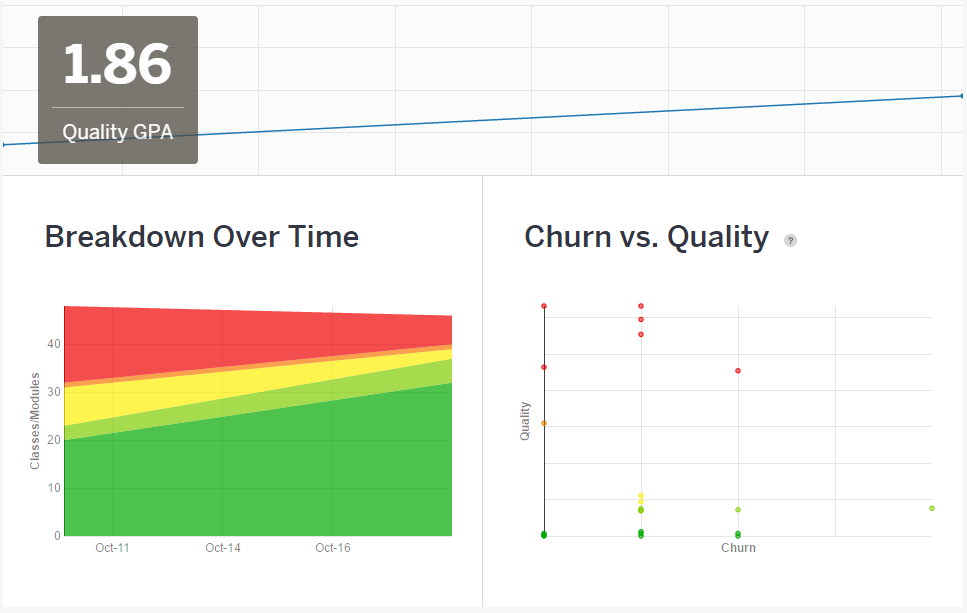
\includegraphics[width=.7\textwidth]{Images/CodeClimate_Beginn.PNG}
	\caption{Code Climate Stand 18.10.2016 - nach der Verfeinerung der Regeln}
	\cite{codeclimate.com}
\end{figure}

Im Verlaufe des Projektes wurden einige Code-Änderungen vorgenommen, welche die Qualität verbesserten. Ein grosses Problem war zum Beispiel, dass einige PHP-Dateien sehr viele Code-Zeilen enthielten und gleichzeitig viel duplizierter Code vorhanden war. Diese Probleme konnten damit angegangen werden, dass der duplizierte Code in separate Funktionen ausgelagert wurde und jeweils auf diese zugegriffen wurde. Dies hat den Vorteil, dass der Code bei Funktions-Anpassungen nur an einem Ort geändert werden muss und nicht an fünf verschiedenen Stellen. Weiter konnten durch diese Massnahme und durch zusätzliche Auslagerungen von Code-Stücken die grossen Dateien in kleinere aufgeteilt werden. \\

\subsection{Stand Projekt-Ende}
Somit konnte die Qualität von 1.86 auf 2.04 gesteigert werden, wie in der nachfolgenden Abbildung ersichtlich ist. Ganz am Ende des Projektes ist jedoch ein kleiner Einbruch zu erkennen. Dies hängt mit der Umsetzung der Datenbank-Änderung zusammen, für welche nur noch wenig Zeit übrig war und kein \gls{Refactoring} gemacht werden konnte.

Die linke, untere Grafik zeigt zudem den Anteil der gut bewerteten Dateien im Verhältnis zu den schlecht bewerteten Dateien an. Hier ist ersichtlich, dass vor allem einige der am schlechtesten bewerteten Code-Stücke leicht verbessert werden konnten.

Auf der unteren, rechten Grafik wird die Qualität ins Verhältnis zu den Anzahl Changes gesetzt, also wie oft eine Datei in der Entwicklung geändert werden muss. Wird eine Datei häufig angefasst, so kann dies ein Indikator dafür sein, dass sie zu viele Funktionen beinhaltet. Als Beispiel kann do.php verwendet werden, welche Abläufe für diverse Seiten unterstützt. Arbeiten mehrere Personen an einem Projekt so ist die Wahrscheinlichkeit gross, dass beide an dieser Datei arbeiten müssen und sich somit in die Quere kommen. In diesem Falle ist der Zugriff hoch. Teilt man do.php nun nach unterstützten Funktionalitäten auf, so lösen sich diese Probleme auf und mit der kleineren Anzahl Zugriffe verbessert sich auch diese Kennzahl. Oben rechts sind die am schlechtesten, unten links die am besten bewerteten Dateien eingetragen. Im Vergleich zum Projekt-Beginn ist auch hier ersichtlich, dass die Qualität einiger Dateien durch die oben beschriebenen Massnahmen verbessert werden konnte.

\begin{figure}[H]
	\centering
	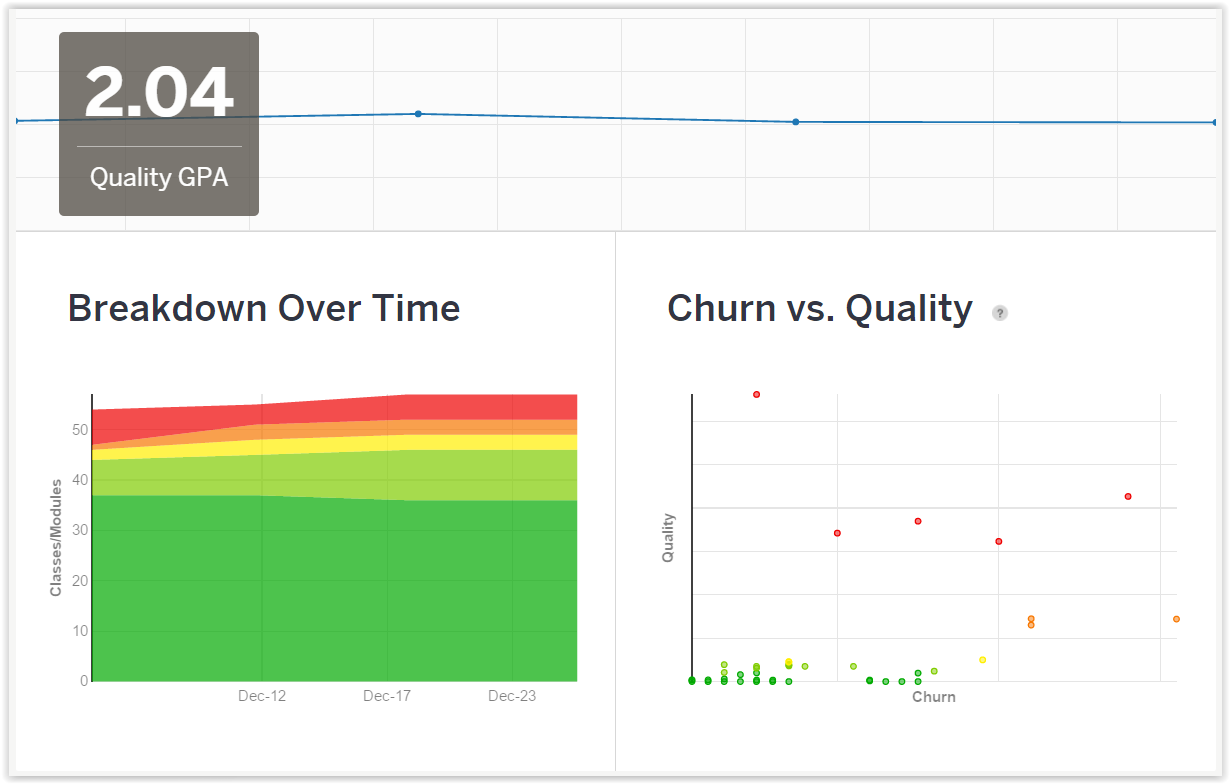
\includegraphics[width=.7\textwidth]{Images/CodeClimate_Ende.PNG}
	\caption{Code Climate Stand 23.12.2016}
	\cite{codeclimate.com}
\end{figure}

Auch wenn die Kennzahlen von Code Climate in diesem Projekt nur selten beachtet wurden, gaben sie gute Hinweise darauf, welcher Code-Stücke noch verbesserungswürdig sind. Es wurde jeweils angezeigt, was das Issue, also das jeweilige Problem, ist und wo es auftaucht.

\begin{figure}[H]
	\centering
	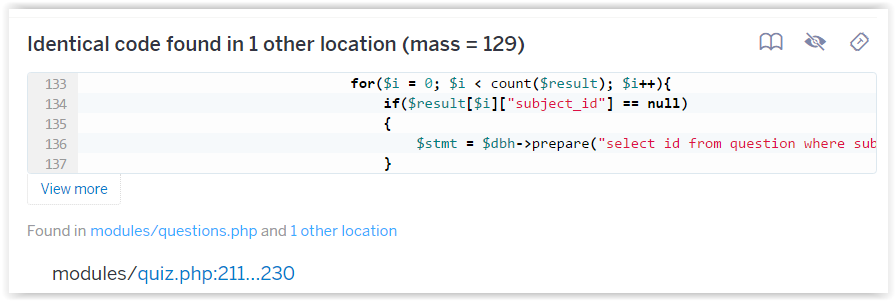
\includegraphics[width=.7\textwidth]{Images/CodeClimate_Issue.PNG}
	\caption{Code Climate - Issue}
	\cite{codeclimate.com}
\end{figure}



\section{Systemtests mit Selenium}
Selenium IDE \cite{seleniumIDE} ist ein Firefox \cite{firefox} \gls{Add-on} für Web-\gls{User Interface}(UI)-Tests. Es ermöglicht das Aufnehmen, die Bearbeitung, das Debuggen und das Abspielen von Tests.
Mit der Hilfe dieses Tools können einfach \acrshort{UI}-Tests durchgeführt werden.

\begin{figure}[H]
	\centering
	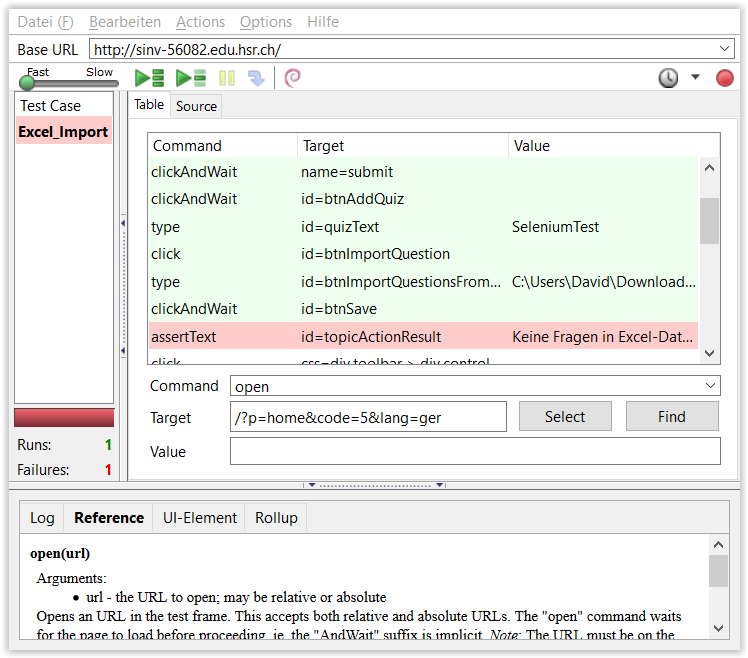
\includegraphics[width=.5\textwidth]{Images/seleniumTest.PNG}
	\caption{Durchführung eines Selenium IDE Test-Case}
\end{figure}

Für die Test-Erstellung genügt es, mit Firefox die Aufgangs-Webseite aufzurufen und auf den roten Aufnahme-Knopf zu drücken. Anschliessend wird die gesamte Navigation auf der Seite aufgezeichnet. Zwischendurch oder ganz am Ende kann dann eine Prüfung mittels \glqq assert\grqq eingefügt werden. Dazu genügt ein Rechtsklick auf das entsprechende Element in der Seite, wie auf dem folgenden Bild dargestellt ist.

\begin{figure}[H]
	\centering
	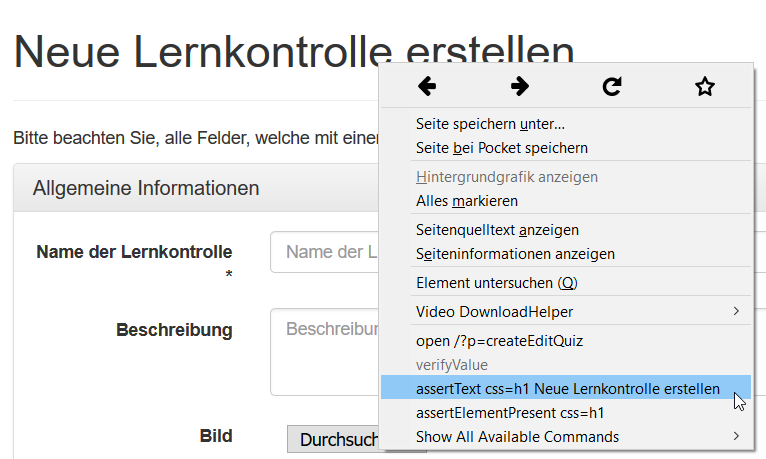
\includegraphics[width=.5\textwidth]{Images/seleniumIDE_Assert.PNG}
	\caption{Erfassung einer Element-Prüfung mittels Selenium IDE}
\end{figure}

Alle erfassten Tests werden abgespeichert und können danach einfach abgespielt werden.

Für diese Arbeit wurden mehrere solcher Tests erfasst. Sie dienten vor allem der Überprüfung beim Durchspielen von sich wiederholenden und gleichbleibenden Fällen, wie dem Erstellen einer Frage. So konnte nach Code-Umstellungen in diesem Bereich geprüft werden, ob noch alle Komponenten korrekt zusammenarbeiten.

Probleme gab es allerdings bei Listenelementen, wie zum Beispiel der Aufführung aller Quizzes. Wählte man ein solches aus, so verwendete Selenium IDE den entsprechenden Index des Elementes in der Gesamtliste. Fügte man anschliessend ein Element zu dieser Liste hinzu oder entfernte eines, so stimmte die gespeicherte Index-Position nicht mehr überein und es wurde beim nächsten Durchlauf des Tests ein anderes Element ausgewählt.

In der Gesamtbetrachtung überwiegen jedoch die Vorteile der einfachen Erstellung und Durchführung der Tests. Weiss man wo die Schwächen von Selenium IDE liegen, so kann es als effizientes Test-Tool eingesetzt werden.


\section{Unit-Tests}
Unit-Tests sind dazu da, einzelne Funktionen zu testen. Wenn eine Basis von Unit-Test bestehen, welche die Funktionalität des Codes abdecken, sind Code-\gls{Refactoring}s leichter umzusetzen. Funktionieren Tests nach dem Umstellen des Codes nicht mehr, so können die Fehler leichter gefunden werden, da die Tests jeweils nur einen kleinen Code-Bereich prüfen.

Zu Beginn war geplant, Unit-Tests mit PHPUnit \cite{phpunit} umgesetzen. Es wäre möglich gewesen, diese Test bei jedem \gls{Commit} automatisch vom Continuous Integration Server Travis CI \cite{travisCI}, ausführen zu lassen. So wäre bei jedem Commit überprüft worden, ob noch alles funktioniert.

Das Problem war, dass der Code in einer nicht-testbaren Form geschrieben war und immer noch ist. Die vorhandenen PHP-Dateien enthalten alle lange Methoden mit vielen Nebeneffekten auf diverse Variablen oder die Datenbank. Somit war es aus zeitlichen Gründen nicht möglich, denn gesamten Code testbar umzuschreiben und entsprechende Unit-Tests zu implementieren.



\section{Continuous Integration}
\acrfull{CI} ist ein Prozess, bei dem die einzelnen Software-Komponenten nach dem \gls{Commit} automatisch getestet und anschliessend mit den anderen Komponenten zusammengefügt werden. Dies bringt den Vorteil, dass die Integration der Komponenten laufend geprüft wird und die Unit-Tests Fehler sofort erkennen. Zudem kann die Code-Qualität anhand von verschiedenen Kennzahlen regelmässig gemessen werden.


\begin{figure}[H]
	\centering
	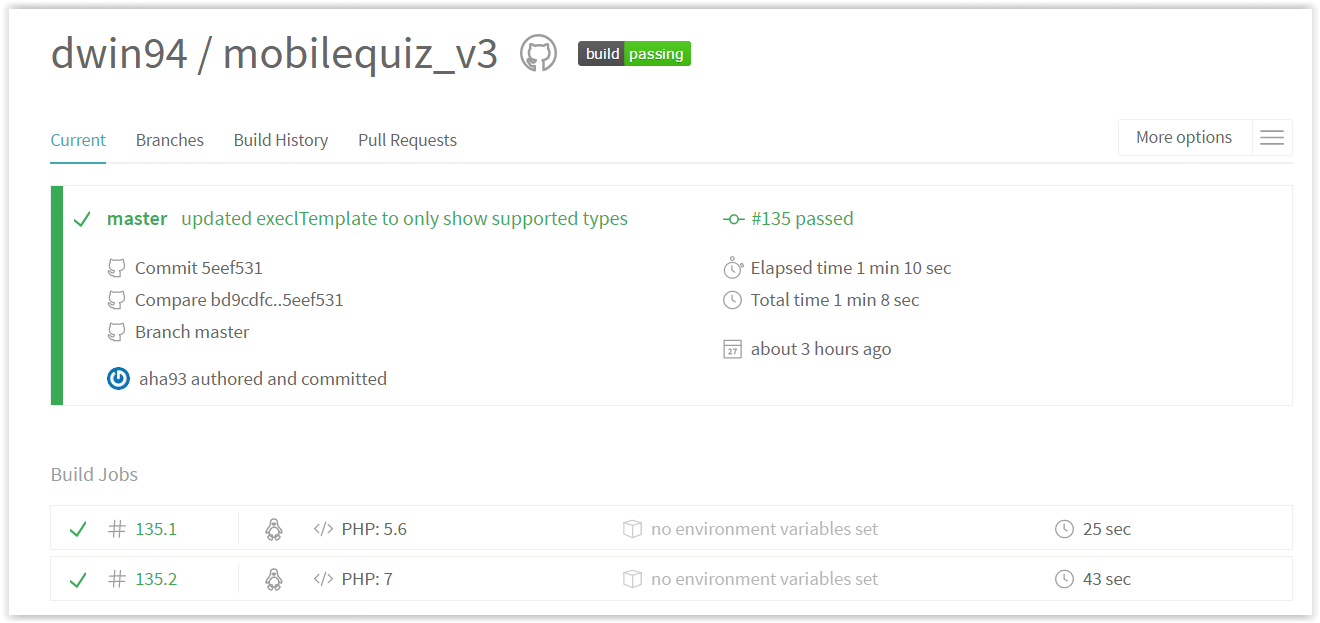
\includegraphics[width=1\textwidth]{Images/travisCI.PNG}
	\caption{TravisCI-Ansicht des letzten Commits}
	\cite{travisCI}
\end{figure}


Dies wurde mit Travis CI \cite{travisCI} teilweise umgesetzt. Unit-Tests waren zwar nicht vorhanden, jedoch prüfte der \acrshort{CI}-Server jeweils die Abhängigkeiten der PHP-Files. Bei erfolgreichem Durchlaufen stiess er zudem das Codestatistik-Tool Code Climate \cite{codeclimate} an, welches anhand von vordefinierten Tests die Code-Qualität mass.
Da die Code-Qualität im Verlauf des Projektes weniger beachtet wurde als zu Beginn war der Einsatz von Travis CI \cite{travisCI} in diesem Projekt eher mehr Aufwand als Ertrag. Das Aufsetzen war aber mit Sicherheit eine gute Übung für ein nächstes Projekt.